% !TeX root = ../main.tex

\section*{Markov Random Fields (MRF)}

\paragraph{Idea:} An image $G$, given by the random matrix $[g_{i,j}]$ can be considered as a pixel grid of random variables.

%Example use cases are denoising, segmentation or stereo matching. 

\begin{equation*}
    p([g_{i, j}]) = \prod_{i,j} p(g_{i, j} | g_{i-1, j} g_{i, j-1} g_{i-1, j-1})
\end{equation*}

\paragraph{Definition of MRF:}
\begin{enumerate}
    \item Positivity:\footnote{For a certain observation the probability is non zero} $ p(\vec{x}_1, \vec{x}_2, \dots, \vec{x}_N) > 0$
    \item Markov property:\footnote{where $\mathcal{N}(\vec{x}_k))$ denotes the neighborhood of $\vec{x}_k$: 1. $\vec{x}_k \notin \mathcal{N}(\vec{x}_k)$; 2. $\vec{x}_i \in \mathcal{N}(\vec{x}_k) \Leftrightarrow \vec{x}_k \in \mathcal{N}(\vec{x}_i)$: 3. $\mathcal{N}(\vec{x}_k) = \{x_i|0 < dist(x_i, x_k) \le t\}$} $ p(\vec{x}_k |\vec{x}_1, \dots, \vec{x}_{k-1}, \vec{x}_{k+1}, \dots, \vec{x}_N) = p(\vec{x}_k | \mathcal{N}(\vec{x}_k)) $
\end{enumerate}


\begin{figure}[H]
  \centering
  \begin{minipage}[b]{0.45\textwidth}
    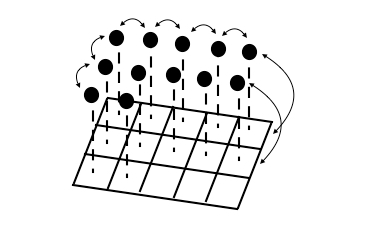
\includegraphics[width=\textwidth]{mrf_image_example}
		\caption{The idea of an MRF on top of an image. The arrows indicate relations (pairwise and between hidden and random variables)}
  \end{minipage}
  \begin{minipage}[b]{0.45\textwidth}
    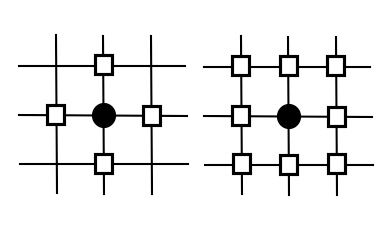
\includegraphics[width=\textwidth]{mrf_grid_neighborhood}
		\caption{4-Neighborhood, 8-Neighborhood (and dynamic-Neighborhood)}
  \end{minipage}
\end{figure}

Two criteria for the hidden variables: 
\begin{enumerate}
	\item Hidden variables that are neighbors should be similar to each other 
	\item A hidden variable should still resemble the original observation (random variable).	
\end{enumerate}

The neighborhoods can also be decomposed in graph Cliques (complete subgraphs) of two. Which is useful later on (factorization + there are solvers for two variables).

\paragraph{Gibbs Random Fields (GRF):} is given by the PDF

\begin{equation*}
	p(x) = \frac{1}{Z} e^{-H(x)}
\end{equation*}

where $Z = \sum_{x^\prime} H(x^{\prime})$ is a partition function and $H(x)$ an energy function, i.e. a sum of potential functions.

%\paragraph{Remark:}
%For a given PDF $p(x)$, the choice of the energy function $H(x)$ is not unique. Consider for example
%
%\begin{equation*}
%	H(x) = - \log p(x) - \log Z
%\end{equation*}
%
%\begin{equation*}
%	p(x) = \frac{1}{Z} e^{-H(x)} = \frac{1}{Z} e^{\log p(x)} e^{\log Z}  = p(x)
%\end{equation*}
%
%$\rightarrow$ we can choose $Z$ arbitrarily\\

\paragraph{Hammersley-Clifford Theorem:} proves that GRFs and MRFs are equivalent. This means we can model the neighborhood relationships in our MRF in terms of the energy and potential functions of the GRF. The first criterium of an MRF is modeled as \underline{pairwise potentials}, the second as \underline{unary potentials} in a GRF.

\begin{equation*}
	p(\vec{x}) = \underset{MRF-probabilities}{\prod_c p_c(\vec{x}_c)} \overset{MRF \Leftrightarrow GRF}{=} \underset{product of potentials}{\dfrac{1}{Z}\prod_c \psi_c(\vec{x}_c)} 
\end{equation*}

Potentials are easier to design, because we are typically interested in the shape of the function (where is it smaller?).

\paragraph{Example:} Image denoising 

Given: The observed noisy image $[g_{i,j}]$ \quad Wanted: Hidden variables are the ideal (noiseless) image $[f_{i,j}]$\\

\textbf{MRF criterium 1:} The ideal image is spatially smooth (pairwise potential).

\begin{equation*}
	p([f_{i,j}]) = \frac{1}{Z} e^{-H([f_{i,j}])}, \quad \text{where } H([f_{i,j}]) = \sum_{i,j} ||\nabla f_{i,j}||_2^2 \qquad (||\nabla f_{i,j}||_2^2 \text{ function of clique of size 2})
\end{equation*}
$ H([f_{i,j}]) $ is sum of squared gradients, computed over a neighborhood (or the sum over all clique potentials).\\

\textbf{MRF criterium 2:} $[g_{i,j}]$ is similar to $[f_{i,j}]$, but corrupted by additive Gaussian noise (unary potential).

\begin{equation*}
	p([g_{i,j}] | f_{i,j}]) = \prod_{i,j} \frac{1}{\sqrt{2 \pi} \sigma_{i,j}} \exp\Big(- \frac{1}{2 \sigma_{i,j}^2} \cdot \underset{\text{energy function $H$}}{(f_{i,j} - g_{i,j})^2}\Big)
\end{equation*}

With these two functions defined, we can solve for a MAP estimate for $f$:

\begin{align*}
	\underset{\text{estimated ideal image}}{[\hat{f}_{i,j}]} &= \argmax_{[f_{i,j}]} p([f_{i,j}] | [g_{i,j}])\\
					&= \argmax_{[f_{i,j}]} \big(p([f_{i,j}] \cdot p([g_{i,j}] | [f_{i,j}])\big)=\dots=\\
					&= \argmin_{[f_{i,j}]} \Big(\sum_{i,j} ||\nabla f_{i,j}||_2^2 + \sum_{i,j} \lambda_{i,j} (f_{i,j} - g_{i,j})^2\Big)
\end{align*}

\paragraph{Solving MRF via graph cuts:} 
The goal is to find an assignment of values to the hidden variables $x_1, \dots,x_N$ that minimizes the energy function:

\[E(x) = \sum_i E^i(x_i) + \sum_{i,j} E^{i,j} (x_i, x_j) \qquad \text{(unary + pairwise potentials)}\]

\underline{Min cut:} smallest possible sum of cut edges that separate s and t $\Leftrightarrow$ \underline{Max flow:} maximum throughput from s to t. We can solve this problem in polynomial time.

A function $\varepsilon(x)$ is \underline{graph-representable}, if there is a graph with configuration $\vec{x}$, so that $\varepsilon(x)$ is equal to the cost of the minimum s-t-cut plus a constant.

If $\varepsilon$ is  graph-representable by G, then we can find an exact minimum of $\varepsilon$ via a \underline{minimum s-t-cut} on G.

Submodular quadratic pseudo-boolean functions are graph-representable. The function for the pairwise potentials needs to satisfy the \underline{submodularity condition}:

\[E^{i,j}(0,0) + E^{i,j}(1,1) \leq E^{i,j}(0,1) + E^{i,j}(1,0)\]

For graph construction we look at minimal subgraphs for both potentials, assign values, compute $E(x)$ and add the subgraphs together (\underline{Additive property}).

\begin{figure}[H]
	\centering
	\begin{minipage}[b]{0.5\textwidth}
		For every term in the Energy function, obtain a subgraph (with s and t). Add up edge weights while constructing final graph. Binary assignment of min cut is optimal solution to MRF minimization problem.
	\end{minipage}
	\begin{minipage}[b]{0.4\textwidth}
		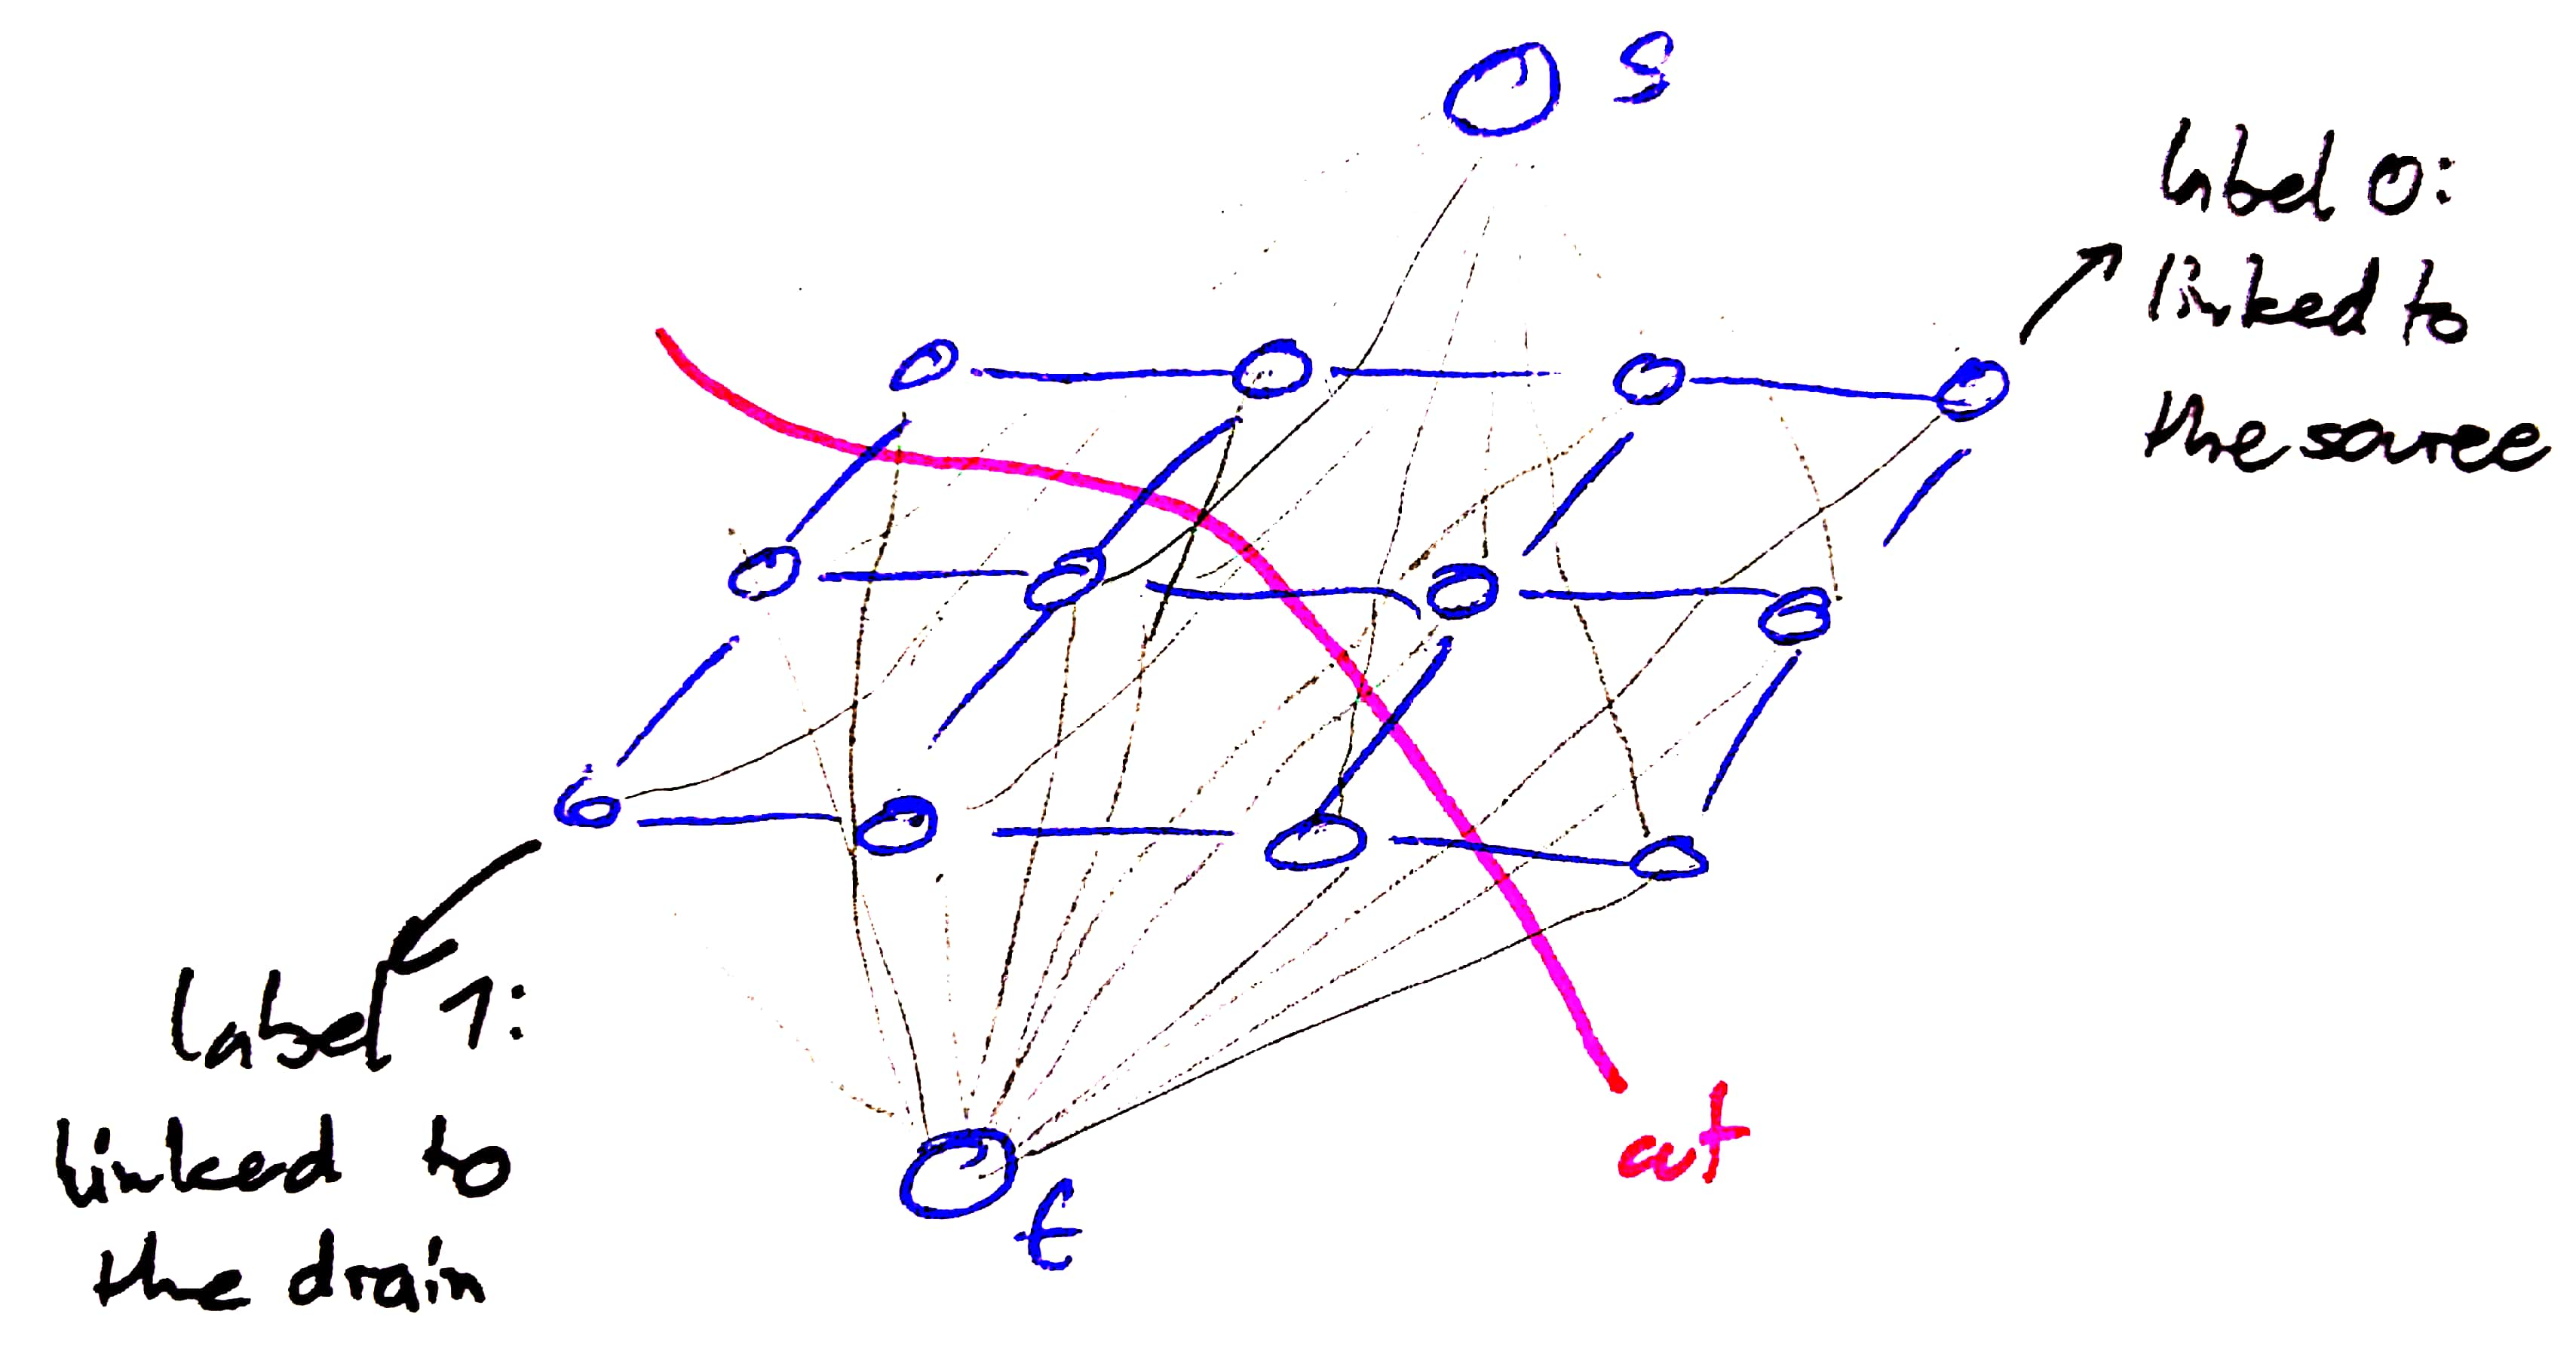
\includegraphics[width=\textwidth]{graph_cut}
	\end{minipage}
\end{figure}

% TODO: Max Flow / Min Cuts


%\bigbreak
%\underline{Max Flow/Min Cut:}
%
%Max Flow: What is the maximum network throughput from source s to drain t? \(\Rightarrow\) use Ford/Fulkerson, or Preflow-Push
%
%Min Cut: Minimum sum of all edges that lead from s to t that are cut to seperate s from t.
%
%Min Cut is also a standard algorithm that runs in polynomial time.
%
%Define: "Graph-representable": A function \(\epsilon (x)\) is graph-representable, if there exists a graph, such that for any configuration \(x\), \(\epsilon(x)\) is equal to the cost of the minimum s-t-cut plus a constant value (which doesnt change for different configurations).
%
%Set \(x_i = 0\) if \(v_i \in S\) (a node is connected to the source), \(x_i=1\) if \(v_i \in \mathcal{T}\) (a node is connected to the drain/sink).
%
%If \(\epsilon\) is graph-representable by \(G\), then we can find an exact minimum of \(\epsilon\) in polynomial time, by computing a minimum s-t-cut on G.
%
%Theorem: Submodular quadratic pseudo-boolean functions are graph-representable.
%
%Submodularity condition on binary label sets: 
%\[E^{i,j} (0, 0) + E^{i,j}(1,1) \leq E^{i,j} (0,1) + E^{i,j} (1,0)\]
%
%We seek to minimize
%\[E(x) = \sum_i E^i(x_i) + \sum_{i,j} E^{i,j} (x_i, x_j)\]
%
%Graph construction:
%See picture
%
%Problem: Find appropriate weights for such a graph.
